% =================================================================================================
% File:			archietettura.tex
% Description:	Defiinisce la sezione relativa a ...
% Created:		2015-02-23
% Author:		Tesser Paolo
% Email:		tesser.paolo@mashup-unipd.it
% =================================================================================================
% Modification History:
% Version		Modifier Date		Change											Author
% 0.0.1 		2015-02-23 			sistemato header								Tesser Paolo
% =================================================================================================
% 0.0.2			2015-03-26			modificata stesura e nuove aggiunte generiche	Tesser Paolo
% =================================================================================================
%

% CONTENUTO DEL CAPITOLO

\section{Descrizione Architettura} % (fold)
\label{sec:descrizione_architettura}

\subsection{Metodo e formalismo di specifica}
La descrizione dell'architettura dell'applicazione viene fornita con un approccio di tipo top-down: si descrive l'architettura partendo dal generale e si analizzano via via in dettaglio tutti i moduli che le compongono. Vengono forniti degli esempi d'utilizzo dei design pattern scelti. I diagrammi delle componenti, delle classi e i diagrammi di attività rispettano il formalismo di UML 2.0. \newline
Librerie esterne usate dall'applicazione verranno marcate con colori diversi per facilitare la distinzione durante la consultazione. \newline
L’architettura generale non tratta l’intero insieme delle sottoclassi del sistema. Di conseguenza viene specificato lo scopo di una gerarchia e vengono individuate le relazioni con le varie componenti del sistema. Il resto dei dettagli viene rimandato alle diverse fasi di Progettazione di Dettaglio.


	\subsection{Architettura generale}
	\label{susb:architettura_generale}
	L’architettura dell'applicazione si ispira all'architettura Three-Tier. Viene quindi suddivisa in tre moduli (detti per comodità anche livelli o tier):
		\begin{enumerate}
			\item Client Tier
			\item Server Tier
			\item DataBase Tier
		\end{enumerate}
		\noindent
		Non si tratta di una vera e propria architettura Three-Tier non essendo applicata a un singolo modulo, e anzi i tre moduli sono distribuiti su macchine diverse. Il riferimento all'architettura Three-Tier è concettuale, ed è servito ai progettisti per pensare alla struttura di base dell'applicazione. Di seguito viene proposto un diagramma rappresentante le relazioni tra i vari livelli. Vengono individuate le componenti che permettono ai vari livelli di interagire senza dover esporre la struttura interna degli stessi. \newline \newline

		\begin{figure}[htbp]
			\centering
			\centerline{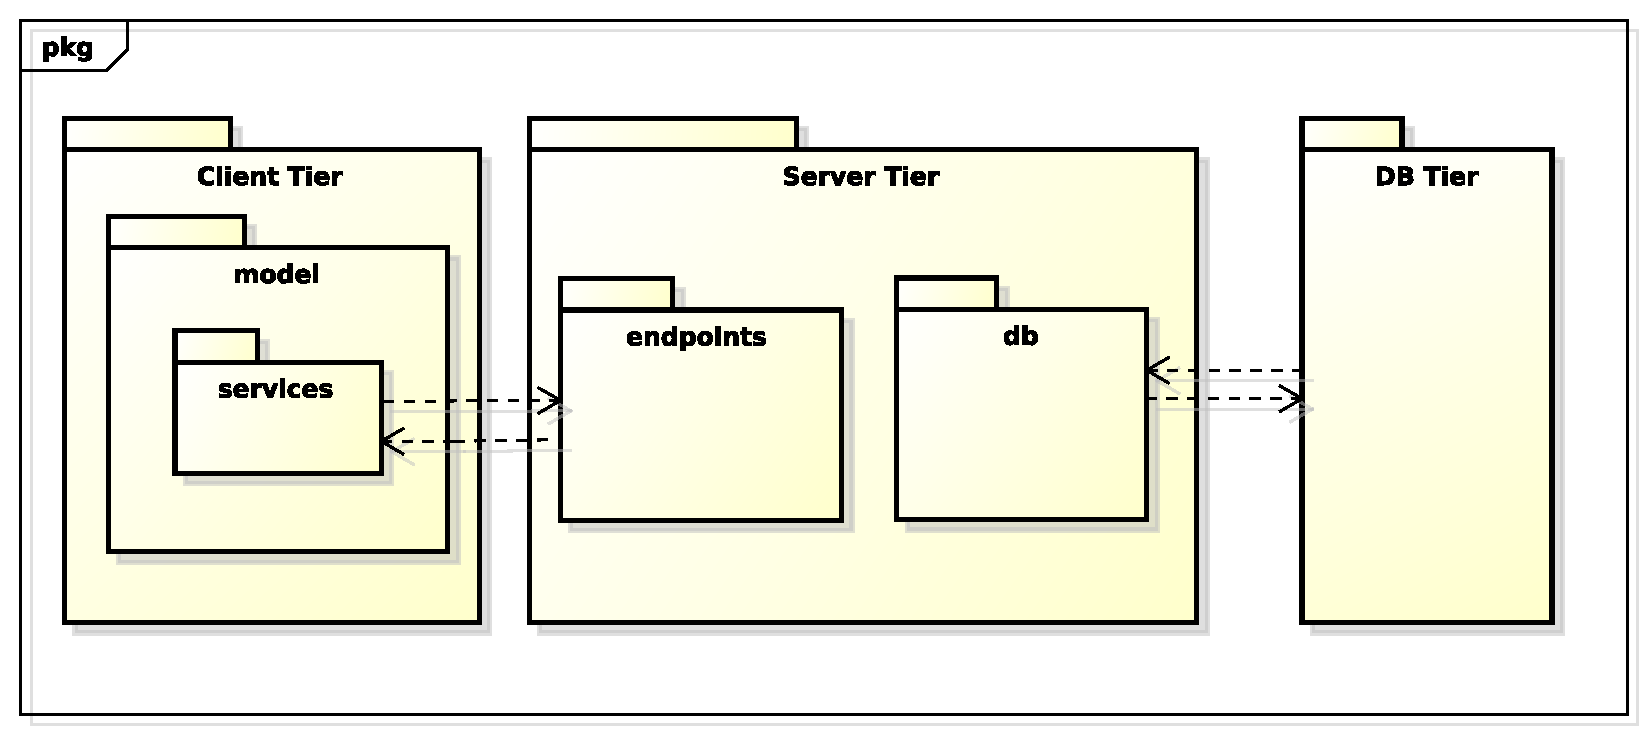
\includegraphics[scale=0.5]{./images/three_tier.pdf}}
			\caption{Three-Tier}
		\end{figure}

		Come indicato nel diagramma, il livello del client interagisce con il server tramite gli Endpoints forniti dal Server. Esso riceverà e analizzerà la richiesta. Una volta pronta, la risposta verrà fornita al Client. \newline
		Il client si occuperà di analizzarla per determinare se la richiesta ha avuto un esito positivo o negativo e nel primo caso utilizzerà i dati per effettuare le opportune operazioni.

		\subsubsection{Architettura Client Tier}
		L'architettura del livello client è stata pensata nell'ottica MVW tipica del framework AngularJS. Questo livello implementa l'interfaccia grafica attraverso la quale utenti autenticati e amministratori possono interagire con il sistema in modo completo.
		\newline
		Gli utenti invocheranno determinate azioni utilizzando i pulsanti forniti dall'interfaccia e il sistema risponderà fornendo pagine di configurazione interattive oppure visualizzando una serie di grafici che verranno aggiornanti costantemente utilizzando i servizi REST forniti dall'applicazione. In dettaglio:
		\begin{itemize}
			\item Model: contiene il modello dei dati e la \textit{business logic}, che comprende le definizioni delle chiamate che può fare l'applicazione e i servizi che offrono. Inserire la logica dell'applicazione nel modello anziché nel \textit{controller} permette di ridurre la duplicazione del codice;
			\item View: contiene tutte le viste utente come astrazione del modello dei dati;
			\item Controller: questo modulo, in AngularJS, espone tutti i metodi forniti dalla logica dell'applicazione e permette l'associazione a due vie dei dati tra il livello astratto nelle viste e il livello concreto del modello.
		\end{itemize}
		\noindent
		Una illustrazione più dettagliata viene fornita nella sezione \ref{sub:client}.

		\subsubsection{Architettura Server Tier}
		Il livello server si occupa di raccogliere i dati grezzi tramite le API fornite dai vari social network, elaborare e salvare tali dati nel database, fornire dei servizi REST ed elaborare le richieste in arrivo dal client. Il back-end è stato suddiviso nei seguenti moduli:
		\begin{itemize}
		  \item db: contiene le definizioni del modello dei dati, sia per quanto riguarda i dati grezzi ricavati dai social network, sia per i dati necessari all'applicativo finale in sé;
			\item miner: contiene le classi ed i package che estraggono i dati grezzi a cadenza regolare e costruiscono nuove entità secondo il modello dei dati che andrà a popolare il database;
			\item processor: rappresenta il punto centrale del back-end. Si occupa di ricevere ed elaborare le richieste provenienti dal client oltre ad avviare il processo di aggiornamento delle Recipe scadute e recupero dei dati grezzi grazie alle funzionalità di \textit{task scheduling} offerte da Google App Engine;
			\item endpoints: contengono le classi che definiscono la struttura dei servizi REST offerti tramite l'utilizzo del servizio Cloud Endpoints reso disponibile dalla piattaforma di Google.
		\end{itemize}
		Una illustrazione più dettagliata viene fornita nella sezione \ref{sub:server}.

		\subsubsection{Architettura Database Tier}
		Il livello database è gestito dal sistema Datastore integrato nella Google Cloud Platform che fornisce la funzionalità di persistenza dei dati. Ad esso spetta il compito di memorizzazione sia tutti i risultati recuperati dal Miner riguardanti i dati grezzi dei social, sia di memorizzare le configurazioni del programma necessarie al Processor e lo stato di lavoro dei Miner ad esso collegati.

		\subsubsection{Protocollo di comunicazione Client-Server}
		La comunicazione tra il livello Client e quello Server avviene tramite i Google Cloud Endpoints. Questi permettono di creare delle API da un'applicazione generata tramite la Google App Engine. Gli Endpoints garantiscono un modo semplice di sviluppare un back-end condiviso, riducendo di molto il lavoro che sarebbe necessario per implementare una simile infrastruttura.


		\subsubsection{Protocollo di comunicazione Server-Database}
		La comunicazione tra il livello Server e quello del DBMS avviene tramite apposite funzionalità messe a disposizione dal servizio Datastore della piattaforma. Per poterle utilizzare il Server dovrà utilizzare il modulo: \textbf{google.appengine.ext.db}.


% section descrizione_architettura (end)
